% adapted by WS from SSR's Word document and from the 5-part series at
% https://www.overleaf.com/learn/latex/How_to_Write_a_Thesis_in_LaTeX_(Part_1):_Basic_Structure
% reviewed by MAM

\documentclass[12pt,twosided]{report}

\usepackage[titletoc]{appendix} % for adding appendix to TOC
\usepackage{biblatex}  % reference management
\usepackage{geometry}  % better margins and margin control
\usepackage{graphicx}  % to include figures
\usepackage{hyperref}  % internal and external links
\usepackage[utf8]{inputenc}  % support for non-ASCII characters
\usepackage{listings}  % typset code
\usepackage{outlines}  % easy nesting of lists
\usepackage{tabularx}  % more control over table column width
\usepackage{titlesec}  % customize chapter title 
\usepackage{upquote}  % prevent mishandling of single quotes in listings
\usepackage{placeins}


% TODO: Customize the appearance of hyperref links using \hypersetup
% See https://en.wikibooks.org/wiki/LaTeX/Hyperlinks#Customization

% Custom format of chapter title.
\titleformat{\chapter}[hang]{\bf\huge}{\thechapter.}{2pc}{}

% Separate folder for images named 'images'.
\graphicspath{ {images/} }

% Separate file for references
\addbibresource{references.bib}

% Replace with your title
\title{The Third Space}

% Allow recalling document title
% from https://tex.stackexchange.com/a/15806/44301
\makeatletter\let\Title\@title\makeatother  

\begin{document}

\begin{titlepage}
  
  \newgeometry{top=100pt,bottom=75pt}   
  \begin{center}
    \vfill
    \textbf{\Huge \Title}
    \bigskip

    {\large Kaavish Report\\
      presented to the academic faculty\\
      by\\\bigskip
      \begin{tabular}{ll}
        Musabbir Abdul Majeed & musabbir.majeed\\
        Syeda Saleha Raza & saleha.raza\\
        Waqar Saleem & waqar.saleem\\
        Abdul Samad & abdul.samad\\
      \end{tabular}
    }\\\vfill
    
\includegraphics[width=.4\textwidth]{logo.pdf}\\
    {\large In partial fulfillment of the requirements for\\
      \textit{Bachelor of Science}\\
      Computer Science\\\medskip
      \textbf{Dhanani School of Science and Engineering}\\\medskip
      Habib University\\\smallskip
      Spring 2020
    }\\\vfill
    Copyright {\scriptsize \textcopyright} 2019 Habib University
  \end{center}
  \restoregeometry
\end{titlepage}

%%% Local Variables:
%%% mode: latex
%%% TeX-master: "report"
%%% End:
  % title page.
\thispagestyle{empty}
\centerline{\textbf{\LARGE \Title}}
\vfill

This Kaavish project was supervised by:\\\bigskip\\\bigskip\\\bigskip

% TODO: Use the appropriate table below depending on whether you have an external advisor. Comment out the unused table.

% If no external supervisor.
\hfill %
\begin{tabular}{l}
  \line(1,0){200}\\
  Nadia Nasir \\ % Name of your CS supervisor
  Faculty of Computer Science\\
  Habib University
\end{tabular}\\\bigskip\bigskip

% % If external supervisor.
% \begin{tabularx}{\linewidth}{lXl}
%   \line(1,0){175} & & \line(1,0){175}\\  % Signatures.
%   My External Supervisor & & My Internal Supervisor \\ % Names of your supervisors
%   Designation & & Faculty of Computer Science\\  % External supervisor's role/job tile at their company.
%   Awesome Ltd. & & Habib University  % External supervisor's company.
% \end{tabularx}\\\bigskip\bigskip

Approved by the Faculty of Computer Science on \hrulefill.

%%% Local Variables:
%%% mode: latex
%%% TeX-master: "report"
%%% End:
  % approval page.

\chapter*{Dedication}
For ammi, abbu and all the hard-working people who try everyday to make the best of their abilities and earn a respectable living. You all are real heros because you know how to fight and live with dignity. May you earn the best of all your dedication and hard-work!

\chapter*{Acknowledgements}
We want to thank the Transgender community of Karachi in helping us get an insight on the distress the minorities communities face on regular basis.\\ We would like to thank the CS faculty for helping us transition

\chapter*{Abstract}
Abstract goes here

% The following are automatically populated by LaTeX \chapter, \section and related, \figure, and \table.
\tableofcontents
\listoffigures
\listoftables

% TODO: Put chapters in a separate folder named 'chapters'.

\chapter{Introduction}
\label{chap:intro}
\section{Problem Statement}

This section explains the problem we are solving and our motivation to do so.

\section{Proposed Solution}

This section gives a summary of our proposed solution, i.e. how does it solve the problem? An overview of the system is provided. A detailed description of each module of the system is presented later in Chapter ~\ref{chap:intro}.

\section{Intended User}

This section outlines the target users of this system. The different types of users in our user base and their interaction with the system are described briefly.

\section{Key Challenges}

This section mentions the key challenges that we foresee in this project and possible ways to address them.

\chapter{Literature Review}
\label{chap:lit}
    
\section{Introduction}

This chapter sheds light on the overarching theme of this project - The Third Space - by looking at the current work done in this particular domain by reviewing academic articles and papers.

As introduced in above sections, this project aims to target two sub domains, i.e. Rights and Employment Opportunities of marginalized communities and market condition(s) of small-scale Arts and Crafts businesses. Therefore, this Literature Review, while taking into account the current state(s) and other similar work that has been done in the area of art and crafts and employment opportunities for marginalized communities, also establishes the novelty of our work by highlighting the differences between the existing work and our work.

This Review will comprise of statistics taken from the cited literature as well as an analysis of primary text. We'll first review the literary sources catering to the domain of the plight of marginalized communities. Followed by this will be the review of the literary sources related to the Pakistani handicraft industry which will then lead to our discussion of rising e-commerce industry in Pakistan.

There are a large number of studies about the transgender communities and much is known and written about 'hijras' (transgender persons) in India, however, very little is documented about them in Pakistan (Jami, 2005). It is also to note that the focus of this research is the sad state of these communities with regards to their rights and employment opportunities, therefore this research will use the umbrella term `transgender' instead of going into the depth of multiple terms ('Zanana', 'Khuwaja Sira', 'Mukhannas', 'Hijra') used within South Asian culture (Winter, 2002). 

\section{Conceptual Frame Work}

This is the high level Conceptual Framework for this project. We have two types of variables here, i.e. independent and dependent variables. The rectangle shaped variables in the given figure are the independent variable while the Eclipse shaped variables are the dependent ones. The relationship between the many variables and the existing research is further discussed in the next sections. 

% \begin{figure}
% %   \caption{Conceptual Framework of the research project}
%   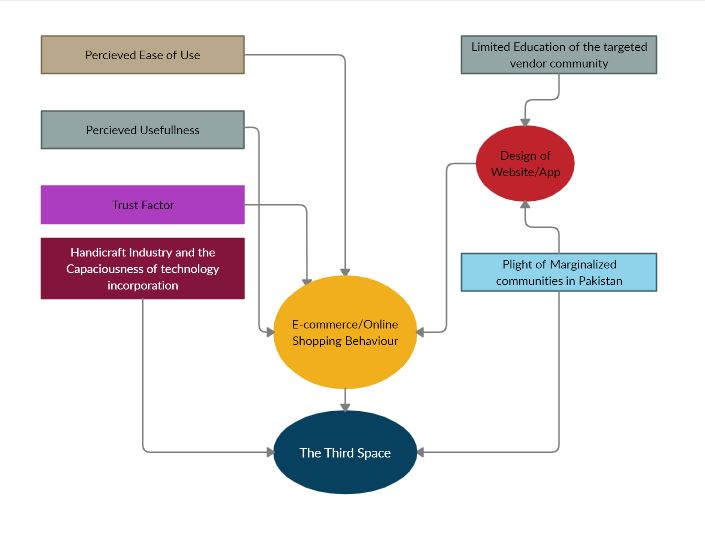
\includegraphics[width=0.75\textwidth]{ConceptualFramework.JPG}
%   \centering
% \end{figure}

\begin{center}
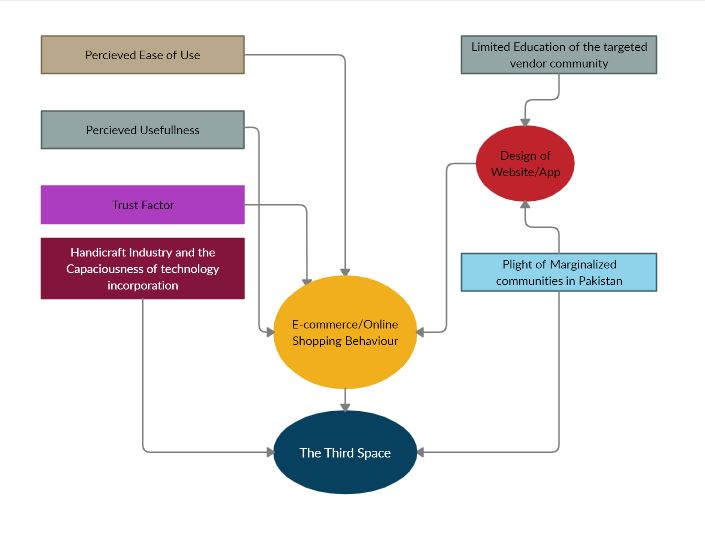
\includegraphics[width=0.75\textwidth]{ConceptualFramework.JPG}
\end{center}



\section{Theoretical Frame Work}

This section discusses the already existing theories and models that comply with the overarching theme of our project. Some of the existing theories that can be considered while reviewing literature for this project includes but not limited to Gender Theory, Technology Acceptance Model (TAM), Task-Technology Fit Model (TTFM), Social Impact Theory, Strategic Networking, information Retrival, Social Construction Theory, Theory of Gender Performativity, Craft Theory, System Theory and Complexity Theory.

\section{Emperical Review of Previous Work(s)}

In this section, we'll look at the research work done already by local and international researchers in the three domains our project is related with. This section will take on these three domains in chronological order and discuss the various researchers' works  and the results they arrived while also putting them in context.

\subsection{The state of Pakistan's marginalized communities}

There is limited literature based on primary data of transgender persons in Pakistan (Nazir \& Yasir, 2016). Just the factor that we have little to no documentation for an entire community in relation to their population, literacy rate, employment rate, etc. is telling enough as to how our society has devoid them of any rights. This is the particular reason why the author(s) of this report chose to work in this domain. The need for this cause to be taken up by scientists and engineers today is far more important so that we can find solutions with the aid of technology and create a better world for all of us. 

In a research done by Jami, H. in 2005 with the name \textit {Condition and status of hijras (transgender, transvestites etc) in Pakistan}, she concludes that,“ `We hate some people but we do not know them and we do not want to know them because we hate them', this dictum stands valid in our attitude towards hijras." This research concludes that the discriminating attitude is in effect by and large in our society against the personalities of transgender communities. It can also be drawn from the study that not only Pakistanis have the instilled bias against the transgender persons and people detest the idea of having a transgender in a family, but they are also considered responsible for sex business and homosexuality (Jami, 2005) both of which in a society as religiously conservative as Pakistan's, are considered blatant sins and is also one of the root causes of violence against the member of these communities. This study also confirms that women tend to have positive attitude towards transgender persons compared to men (who are also the performers and executers of violence on the members of this already marginalized community). 

Another research done by Tabassum, S. \& Jamil, S. in (2014) by the title of \textit {Plight of marginalized: Educational issues of transgender community in Pakistan} also affirms the same as Zubaida (a trans woman) states “Brothers and fathers never bother to think about our (transgender person) situation perhaps they thanked to God if we left the home”. Tabassum \& Jamil also concludes in their study that there is a greater desire (of almost 94\% of the sample population from the community) to acquire education and it's their belief that education is a necessary tool for their upwards mobility. However, it was also gathered that some of them who tried to get education faced lot of problems in terms of their enrollment in schools, group selection in the class rooms and in answering the unknown questions of the fellows (Tabassum, S., \& Jamil, S., 2014). 

The findings from the research conducted by Nazir, N., \& Yasir, A. in 2016 in the northern province of Pakistan by the title \textit {Education, Employability and Shift of Occupation of Transgender in Pakistan: A Case Study of Khyber Pakhtunkhwa.} showed that transgender people have experienced unemployment twice the rate of the population as a whole. 97\% of the surveyed population was facing mistreatment on the job. Out of total 47\% faced an adverse job outcome, including job refusal, or being fired or denied promotion. 26\% lost their job because of being transgender. 15\% of the sampled respondents lived in poverty which was double the rate of the general population (Nazir \& Yasir, 2016). This study also talks about the stigma attached to the families of transgender persons and how society continuously taunts them till they disown their child which leads them to being deprived of normal life, education and later on earning means that are considered honorable in the society (Nazir \& Yasir, 2016). It is also to note that this report also talks about the landmark judgment by the Supreme Court of Pakistan which directed both federal and provincial governments to ensure the rights of education, employment and inheritance (Nazir \& Yasir, 2016). Yet, the measures taken by the state in accordance with the court's ruling are not concrete enough to provide the support they need.

Contextualizing the above findings of all of these reports, we can easily draw the conclusion that the community under consideration is one of the many marginalized communities in our society and there are various factors acting behind this sad state of affairs. Therefore, the need for such a project which could create employment opportunities for them is due well in time.

\subsection{The state of Pakistan's handicraft industry}

We begin by deconstructing the term 'handicraft'. Different researchers have described it didfferently. For example, Fabeil (2014) describes that Handicraft refers to handmade products that have artistic and cultural attraction based on their material, design and workmanship. Whereas, Rogerson (2010) attests that craft products should be eighty percent (80\%) made by hands that may include various raw materials such as natural fibers, textiles, beads clay and recyclable materials. However, Thompson (1995) and Abryareh (2006) defines handicraft as a skill, specifically involving practical arts. Most of the debate about definition is on how product is made (handmade versus machine-made, simple versus artistic qualities etc. but the understanding of it as a means of cultural preservation and money-generating economic option is established.

The handicraft sector plays a vital role in income and employment generation and has also been recognized worldwide as a tool for poverty reduction (Allal \& Chuta, 1982). It is a means of preserving and promoting cultural and artistic traditions, such as various techniques and skills of traditional crafts are transmitted from generation to generation. For many countries, the significant unique cultural heritage is retained in their handicrafts, concluded Allal, M., \& Chuta, E. in 1982 in their research by the title \textit {Cottage industries and handicrafts; some guidelines for employment promotion.}

In an extensive study undertaken by a team of British Council (a worldwide cultural organisation of United Kingdom) with the title of \textit {Mapping cultural and creative industries in Pakistan}, the handicraft industries in context with Pakistani society is looked upon in depth. It is concluded in the study that although handicrafts lie in the hemisphere of culture and creativity, the idea of culture and creativity being an evolving industrial activity with wider social, economic and cultural impacts is one which has developed over a long period of time.

In another research by Yang, Y., Shafi, M., Song, X., \& Yang, R. in 2018 by the title of \textit {Preservation of cultural heritage embodied in traditional crafts in the developing countries. A case study of pakistani handicraft industry}, the rise and fall of Pakistani handicraft making as an industry and the impact(s) of technological advancement on this sector. The handicraft trade at global level is focused on customer’s needs and tastes instead of trade in culture. The production of handmade products in bulk quantities, requires mechanical support for finishing and processing. Moreover, the artisan needs to produce innovative designs, shapes, color etc. to match the needs of customers and such innovation may not contain traditional flavor. In Pakistan, several studies indicate that handicraft producers have a low level of education. One of the major reason of low education is that various products require complex and lengthy process and often involves whole family including children which means children quit or miss the school. This is one of a challenging constraint in preserving craft tradition as low level of education makes it difficult for artisan to access various government schemes, obtain market information, bargain with middlemen/traders and manage business properly, thus making them uncompetitive. Moreover, the number of vocational institutes providing training in handicraft skills is very small in various countries such as the case of Laos, there is only one vocational training school (Yang, Shafi, Song, \& Yang, 2018). It is also to note  that the handicraft industry is considered as a low technology sector which involves traditional methods of production and designs. According to prior studies, the handicraft producers lacked the capability to design and develop new products, therefore they are unable to create the marketable product.

Nowadays, customers have rapidly changing demand for new designs; in order to compete in market, the crafts worker should understand the changing needs of customers and should introduce modern designs, however, the traditional design motif should be preserved. Due to lack of innovation and technology the artisans are unable to meet the demands of the customers (Yang, Shafi, Song, \& Yang, 2018). The innovation is a transformation of ideas and knowledge into new products or services which involve technology and the organization, and can be in terms of production, services, processes or management (Ramadani, \& Gerguri, 2011). Culture can also be preserved through innovation in small businesses (Dana, 1999). As a result, entrepreneurs play a crucial role to ensure that the handicraft industry and its cultural identity are preserved for future generations. Even though the human interaction cannot be simply replaced by the technology, there is significant scope to develop activities that not only document and preserve the knowledge of craftsmanship but also ensure the transmission of this knowledge to younger generations. Moreover, in order to enhance the productivity and efficiency of craft production, technology can be used. Using technology, another way to distinguish handicraft products is to put story behind the unique features, the way it is made, origin of product’s design or the artisans and their culture. Such stories can be attached through digital marketing techniques. This will not only help to distinguish, improve sales but will also help to increase the value of product due to its uniqueness from other substitute products. In addition, it is also one of best way to educate customers about the crafts.

In her thesis report, \textit {The Contemporary Value Chain}, Zahra, S. Virsa also concluded that one of reason behind decline in Pakistani handicraft industry is the lack of innovation in design and emphasized that artisans should adopt modern tastes of customers to compete in the market. Also, there is a wide gap of cooperation between designers and artisans, the designers have the professional knowledge and knowhow about the modern taste and artisans have cultural heritage skills and knowledge, thus their cooperation can lead to expansion of business and competitiveness.

In light of the above-mentioned works, it can be seen that the need of amalgamation of craft industrywith technology can actually pull off a competitive and profitable entrepreneurial venture, which our project aims to be.




\subsection{The state of Pakistan's rising E-commerce}

'Since fake e-stores, cybercrimes and scam websites are very common in Pakistan, people hesitate to shop online.' (Adnan,  2014, p.1). The paradoxical state of Pakistani E-commerce industry is self-explanatory as to what factors are contributing the most in the online consumerism. The study conducted by Adnan, H. in 2014 by the title of \textit {An analysis of the factors affecting online purchasing behavior of Pakistani consumers}, concludes that trust deficit is the most important hinderance in Pakistani neonate E-commerce industry. It also points out that lack of accountability and the presence of con artists and vultures in the cyber world have resulted in unpleasant experiences of online Pakistani shoppers. It is also concluded that while the quality of the website had a significant positive relationship with purchase intentions, Pakistan’s online stores should build strategies to better address reliability and trustworthiness issues instead of merely focusing on website design, aesthetics and content factors (Adnan, 2014).

Connecting the two, craft industry and e-commerce, in another study undertaken by Batchelor, S. J., \& Webb, M. in 2002 by the title of \textit {E-commerce options for third world craft producers}, the authors discussed at length the challenges which developing countries face in general as they prepare for e-businesses. In addition to this, the nature of handicrafts and crafts markets bring their own specific barriers and constraints for artisan producers who want to sell direct to end consumers (Business to Consumer, (B2C)). To name a few, the study points out 6 barriers the handicrafts market brings to e-commerce. These include (1) ‘You can see, but you cannot touch, feel and smell’, (2) Digital photographs being not colour accurate, (3) Consumers expect high service standards, (4) Trust factor, (5) Financial Security, (6) Personal Data and Privacy.

The similar study suggests that there are opportunities for improving the supply chain of existing handicrafts through Information and Communication Technologies (ICT).There are some opportunities for ‘digital crafts’ using the Internet to protect indigenous knowledge and create income streams from it. It also suggests some key strategies for an e-commerce website. It rightly points out that the target audience(s) will determine style, language and type of information; as well as what information you present about your organization on your platform. It also suggests to integrate and register with search engines and optimise ranking while also posing the question of “the 5 W's and the H”. It also rightly concludes that the web offers the opportunity to start small, get feedback from users (either directly, or indirectly from site usage logs), and to develop services and facilities incrementally according to need.

Now we delve into the technical aspect of building an e-commerce website by reviewing the relevant literature.

\subsubsection {Technological aspects of E-commerce}

In order to look at the technical details of websites, we reviewed certain academic articles and the pattern we could see was that a lot of studies focused on the front-end of the website (the part of website that interacts with the end user) because of its interactive nature. According to Song, J., \& Zahedi, F., in a research study \textit {Web design in e-commerce: a theory and empirical analysis} in 2001 in which they talk about the key languages to be used in a website that cotributes to the interactiveness of the website, in a result maintaining a larger flow of audience to the website. The languages, libraries and frameworks like HTML5, CSS3, JavaScript, jQuery and PHP were considered appropriate for the development as HTML5 new features allowed the Website to become extremely interactive, CSS3 transitions and animations smoothed the User Interface of the application, JavaScript and jQuery technologies are used to capture the events triggered by the user, PHP scripting language is used to perform server side requests needed to generate emails and objects are saved into the database using JSON file format and managed with PHP and SQL queries.

In another review, \textit {An integrated approach for developing e-commerce applications} by García-Sánchez, F., Valencia-García, R., \& Martínez-Béjar, R. in 2005, the authors discussed the usage of MySQL Database Server because, apart from being Open Source (uses the GPL—GNU General Public License), it is very fast, reliable, and easy to use MySQL Reference Manual (2002). Also, the MySQL Database Software is a client/server system that consists of a multi-threaded SQL server that supports different backends, several different client programs and libraries, administrative tools and a wide range of application programming interfaces (APIs).

Based on the above literature review, it seems reasonable to conclude that research on individual customer’s evaluation and use of e-commerce websites has mainly taken a cognitive perspective though higher-order affective constructs have been paid certain attention. Primitive affective constructs that may underlie higher-order affect and cognitive processes have been overlooked largely though a few constructs (e.g., perceived visual attractiveness, perceived aesthetics) capturing primitive reactions have been proposed. It is important to note, howeverm that both perceived visual attractiveness and perceived aesthetics are primitive constructs.  (Li, N., \& Zhang, P., 2005).

\section{Summary of Literature}

As discussed in detail in this Literature Review, the three major domains that this project lies in, i.e. the employment problems of the marginalized communities, the condition and opennes of handicraft industry, and the rising yet less-equipped E-commerce industry, of Pakistan have been worked upon by multiple national and international researchers. The academic work present however, do not talk about the intersection of all three domains as such. The work done on the intersection of the latter two topics is also present but there persists a knowledge gap when we look at the first research domain, i.e. the employment problems of the marginalized communities in relation with the latter two. This document has tried to look at all the three domains in relation with each other to form a better understanding of the theme of the project itself. This is also to note that in the existing literature the variable of performing arts in relation with e-commerce isn't discussed at all, which is one of the aim of this project at a fairly later stage. 

We are not winding-up the review on any definite perspective as this document is a work-in-progress and will continue to update over the course of 2019 and 2020 till this project continues. The literature to be reviewed can further be expanded or contracted based on the evolution of the project. 
\section{References}

\begin{itemize}
     
\item Jami, H. (2005, July). Condition and status of hijras (transgender, transvestites etc) in Pakistan. In Sexualities, Genders and Rights in Asia’, 1st International Conference of Asian Queer Studies Retrieved September (Vol. 5, p. 2006).

\item Sharma, S. K. (2000). Hijras: The labelled deviance. New Delhi: Gyan Publishing House.

\item Talwar, R. (1999). The third sex and human rights. New Delhi: Gyan Publishing House

\item Winter, S. (2002). Transgender Asia. Retrieved June 21, 2004 from http://web.hku.hk/~sjwinter/TransgenderAsia/index.html

\item Nazir, N., \& Yasir, A. (2016). Education, Employability and Shift of Occupation of Transgender in Pakistan: A Case Study of Khyber Pakhtunkhwa. Dialogue (Pakistan), 11(2).

\item Tabassum, S., \& Jamil, S. (2014). Plight of marginalized: Educational issues of transgender community in Pakistan. Review of Arts and Humanities, 3(1), 107-122. 

\item CSS Forum. (2010). Why is there no Status of the Third Gender in Pakistan. Retrieved from http://www.cssforum.com

\item Allal, M., \& Chuta, E. (1982). Cottage industries and handicrafts; some guidelines for employment promotion. International Labour Office.

\item Abryareh, R. (2009). Tourism Attractions and their Influences on Handicraft Employment in Isfahan. Master’s Thesis, Lulea University of Technology.

\item Simon, T. Miranda. (1995). The Craft of Functional Programming; Addison-Wesley Longman Publishing Co.

\item Rogerson, C.M. (2010). The Enterprise of Craft: Constraints and Policy Challenges in South Africa. Acta Acad. 42, 115–144.

\item Fabeil, N.F., Pazim, K.H.; Marzuki, K.M.; Langgat, J. (2014). The orientation of handicraft entrepreneurs in Sabah: Their personality characteristics and motivations (Orientasi Usahawan Kraftangan di Sabah: Ciri Personaliti dan Motivasi). In Proceedings of the 2nd ASEAN Entrepreneurship Conference, Penang, Malaysia.

\item Fatori´c, S., Seekamp, E. (2017). Securing the Future of Cultural Heritage by Identifying Barriers to and Strategizing Solutions for Preservation under Changing Climate Conditions. 

\item Simon, T. Miranda. (1995).The Craft of Functional Programming; Addison-Wesley Longman Publishing Co.

\item Ramadani, V. \& Gerguri, S., (2011).  Theoretical framework of innovation: Competitiveness and innovation program in Macedonia.

\item Zahra, S. Virsa, (2015). The Contemporary Value Chain. Master’s Thesis, Virginia Commonwealth University.

\item Dana, L.P. (1999). Preserving culture through small business: Government support for artisans and craftsmen in Greece. 

\item Yang, Y., Shafi, M., Song, X., \& Yang, R. (2018). Preservation of cultural heritage embodied in traditional crafts in the developing countries. A case study of pakistani handicraft industry. Sustainability, 10(5), 1336. https://www.mdpi.com/2071-1050/10/5/1336

\item Evans, K., Stockley, S., Taylor, C., Brown, J., Rab, M., \& Khan, S. (2014). Mapping cultural and creative industries in Pakistan. 

\item Adnan, H. (2014). An analysis of the factors affecting online purchasing behavior of Pakistani consumers. International Journal of Marketing Studies, 6(5), 133.

\item Batchelor, S. J., \& Webb, M. (2002). E-commerce options for third world craft producers. UK Department for International Development (DFID).

\item Muhammad, T., \& Kim, K. M. (2018, April). Sustainable and ICT-Enabled Development in Developing Areas: An E-Heritage E-Commerce Service for Handicraft Marketing. In Journal of Physics: Conference Series (Vol. 989, No. 1, p. 012009). IOP Publishing.

\item Song, J., \& Zahedi, F. (2001). Web design in e-commerce: a theory and empirical analysis. ICIS 2001 Proceedings, 24.

\item García-Sánchez, F., Valencia-García, R., \& Martínez-Béjar, R. (2005). An integrated approach for developing e-commerce applications. Expert Systems with Applications, 28(2), 223–235. doi:10.1016/j.eswa.2004.10.004 

\item Li, N., \& Zhang, P. (2005). Toward e-commerce website evaluation and use: an affective perspective. In Post-ICIS 2005 JAIS Theory Development Workshop, Las Vegas, NV.

\item Tan, W., Fan, Y., Ghoneim, A., Hossain, M. A., \& Dustdar, S. (2016). From the Service-Oriented Architecture to the Web API Economy. IEEE Internet Computing, 20(4), 64–68. doi:10.1109/mic.2016.74 


\end{itemize}
%Of course, we take inspiration from \cite{einstein} but wish the work was typeset in \LaTeX \cite{knuthwebsite}, e.g. by taking help from \cite{latexcompanion}.%

\chapter{Software Requirement Specification (SRS)}
\label{chap:srs}
This chapter provides detailed specifications of the system under development.

\section{Functional Requirements}

This section describes each function/feature provided by our system. These functions are logically grouped into modules based on their purposes. The users in our system are categorized as client (is able to sell), customer (is able to buy) and administrator.

\subsection*{Module 1: Registrations}
\begin{outline}
    \1 \textbf{Function 1: Register an account} \\
    The system lets users register an account on the website as a client and as a customer.
        \2 \textbf{Function 1a: Register as a client} \\
        The register form prompts the user to enter their details i.e. Name, Email, Password. The form is submitted and an unverified client account is created. The user receives a link on their email address which completes account verification.
        \2 \textbf{Function 1b: Register as a customer} \\
        The register form prompts the user to enter their details i.e. Name, Email, Password. The form is submitted and an unverified customer account is created. The user receives a link on their email address which completes account verification.
\end{outline}

\subsection*{Module 2: Buying and Selling}
\begin{outline}
    \1 \textbf{Function 1: Only client type users can upload item(s) to sell} \\
    A registered client can upload an item to sell through the mobile application. The system prompts the client for item photos, item category and item details and the item is added to the item inventory.
    \1 \textbf{Function 2: Add item to cart} \\
    A certain button on the item page prompts the system to add the item to the user's cart. All consequent item(s) added without checkout, are added to the same cart unless cleared.
    \1 \textbf{Function 3: Clear item from cart} \\
    The system allows the user to remove a previously added item from the cart. If cart is empty, the checkout link is no longer accessible.
\end{outline}

\subsection*{Module 3: Order Handling}
\begin{outline}
    \1 \textbf{Function 1: Place an order} \\
    The system allows the user to checkout when there is one or more quantity of item(s) in the cart. The checkout button prompts the system to do a user check. The next operation depends on whether the user is registered or unregistered. Once an order is placed, the client for the particular product(s) receives notifications with the order details and a suitable time-frame.
        \2 \textbf{Function 1a: Place order as a registered user} \\
        The system requests the user to enter new, or choose preexisting billing and delivery information. The order is then placed and assigned a unique order number for later use.
        \2 \textbf{Function 1b: Place order as an unregistered user} \\
        The system requests the user to register. The process in Module 1, Function 1b is carried out. This is followed by the system prompting the user for billing and delivery information. The order is then placed and assigned a unique order number for later use.
    \1 \textbf{Function 2: Cancel an existing order} \\
    The system lets a user cancel an existing order if it is not yet dispatched. The system checks the status against the order number. If it meets the case, the order is removed from the database and the client receives notifications of order cancellation.
    \1 \textbf{Function 3: The user can provide different billing and shipping addresses for an order}\\
    The system lets user decide billing and shipping addresses differently, with older ones as default selected option(s). The system stores the order such that once it is billed for, it is delivered to the recipient.
\end{outline}

\subsection*{Module 4: Delivery System}
\begin{outline}
    \1 \textbf{Function 1: Customer and client are notified of order delivery status} \\
    The client is notified of an incoming order and it is stored in their portal as an ongoing order, not yet collected. Once collected by the rider, it is confirmed as such. The admin receives the notification and is prepared to receive the order for quality assurance. Once it leaves the admin, the user is notified that the order has been dispatched and is to be expected. The user receives the order, it is confirmed by the rider, and the order delivery is complete.
\end{outline}

\subsection*{Module 5: Admin Portal}
\begin{outline}
    \1 \textbf{Function 1: Admin can remove items from the database} \\
    If a certain item does not fit the website's criteria for product, admin can remove it from the website. The client is notified that the order has been removed since it does not comply with our standards.
\end{outline}
\subsection*{Module 6: User Account Portal}
\begin{outline}
    \1 \textbf{Function 1: User can change billing and shipping information} \\
    Previous billing and shipping address can be deleted. The system removes information from its database. User can then choose to add a new set of information that is updated in our database.
    \1 \textbf{Function 2: User can change notification settings}
        \2 \textbf{Function 2a: Promotional notifications can be turned off} \\
        User notifications for promotions are sent via email. They can be turned off via the portal. User is removed from mailing list. Upon next login session user is reminded to turn on their promotional emails.
        \2 \textbf{Function 2b: Order notifications must be turned on for at least one medium} \\
        User receives order notifications through email and phone. This can be turned off through the portal, however, user must have at least one active notification medium for orders.
    \1 \textbf{Function 3: User can retrieve order history} \\
    User can access order history through account portal. The order contains details relevant to order.
\end{outline}

\subsection*{Module 7: Shop Handler}
\begin{outline}
    \1 \textbf{Function 1: Registered clients can create a shop} \\
    On account registration as a client, system responds with a page where client can create a shop. Shop handles all client data with regards to buying and selling products. The shop creation requires the client to enter a Name, Address and Phone Number. The system verifies the shop upon admin approval, and clients can then start selling.
    \1 \textbf{Function 2: Registered clients can change shop details} \\
    The client can change shop address and number through the shop portal inside their account. This cannot be done during an ongoing order on the current shop. Once all orders from the current shop are delivered, only then client can change shop details.
\end{outline}

% --- The above is to be modified as per your project, e.g. a flat list if your system has limited functional requirements.

\section{Non-functional Requirements}

\subsection*{Performance:}
\begin{outline}
    \1 Response time should not exceed 12 seconds for all pages and 7 seconds for the landing page
    \1 System should be able to handle 250 users simultaneously
    \1 50 simultaneously placed orders should be handled without crashes and errors
\end{outline}

\subsection*{Interface:}
\begin{outline}
    \1 Client should be able to upload an item to sell in 3 steps
    \1 Website and Mobile Application should have consistent color scheme
\end{outline}

\subsection*{Resource:}
\begin{outline}
    \1 Mobile Application should run without lag on 1 MB RAM smartphones
    \1 Quality Assurance requires a physical space for order handling
    \1 Quality Assurance requires personnel
\end{outline}

\subsection*{Verification:}
\begin{outline}
    \1 Email verification API should be deployed
    \1 Client has to be verified through contact before email verification
\end{outline}

\subsection*{Documentation:}
\begin{outline}
    \1 Version control maybe supplemented by proper documentation of the versions
\end{outline}

\subsection*{Security:}
\begin{outline}
    \1 User login session has to expire after 24 hours
    \1 Payment and all user information is encrypted
\end{outline}

\subsection*{Portability:}
\begin{outline}
    \1 Database backup must be maintained every 10 days
\end{outline}

\subsection*{Quality:}
\begin{outline}
    \1 Product placed on the website must have equal to or more than 3 images
    \1 Item(s) with orders more than 3 and rating less than or equal to 2.5 is reviewed
    \1 More than 90\% of user testing should be positive 
\end{outline}

\subsection*{Maintainabilty:}
\begin{outline}
    \1 New version must contain all older information
    \1 Code should allow for easy new module integrations
\end{outline}

\subsection*{Usability:}
\begin{outline}
    \1 Client survey after 2 months should have a usability score of 8/10 or more
\end{outline}

\section{External Interfaces}

\subsection{User Interfaces}
We have created an interactive dummy mobile app which is accessible through this link: https://marvelapp.com/jaefbg9/screen/62586242

\subsection{Application Program Interface (API)}
The APIs used for our system will be: 
\begin{outline}
    \1 Google Recommendations API (subject to change)
    \1 Social Login
    \1 Email Sender
    \1 User Authentication API by PassportJS
    \1 Facebook API
\end{outline}

\subsection{Hardware/Communication Interfaces}
For \textbf{Hardware Interfaces}, the Web Application would require hardware used to connect to the internet. The Mobile Application would require hardware that supports Android Operating System and internet connectivity. \\ For \textbf{Communication Interfaces}, we will be using the HTTP and TCP/IP protocol.

\section{Use Cases}
This section presents detailed use cases of our system.\\
\begin{figure}
  \caption{UseCase 1: Vendor Registration}
  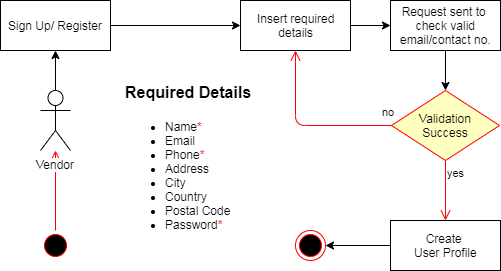
\includegraphics[width=0.75\textwidth]{Vendor_Registration.png}
  \centering
\end{figure}
\begin{figure}
  \caption{UseCase 2: How to Create a Shop}
  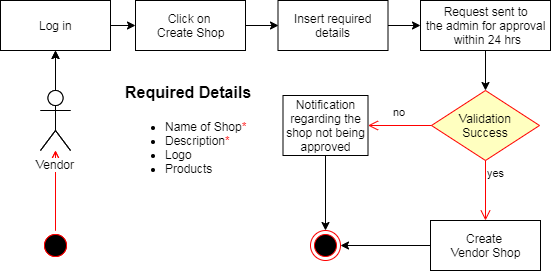
\includegraphics[width=0.75\textwidth]{Shop_Creation.png}
  \centering
\end{figure}
\begin{figure}
  \caption{UseCase 3: Upload a New Product}
  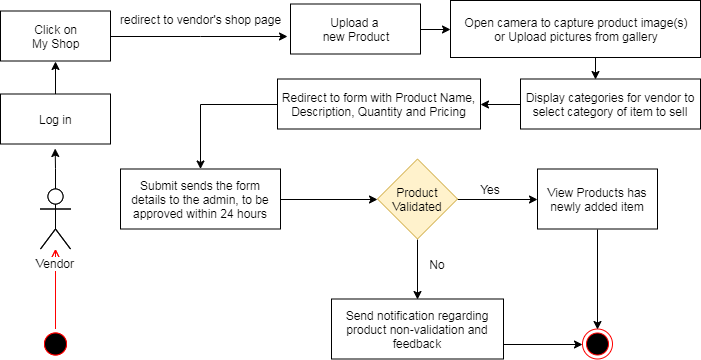
\includegraphics[width=0.75\textwidth]{UploadAProduct.png}
  \centering
\end{figure}
\begin{figure}
  \caption{UseCase 4: Edit/Update an existing Product}
  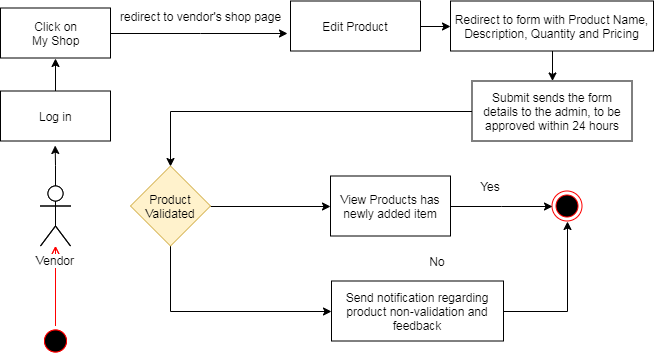
\includegraphics[width=0.75\textwidth]{EditMyProduct.png}
  \centering
\end{figure}
\begin{figure}
  \caption{UseCase 5: Get notified of new orders}
  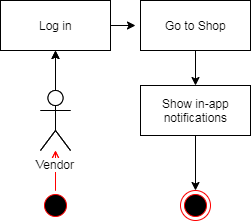
\includegraphics[scale=1]{OrderActivityNotification.png}
  \centering
\end{figure}
\begin{figure}
  \caption{UseCase 6: Create (and keep updating) your blog}
  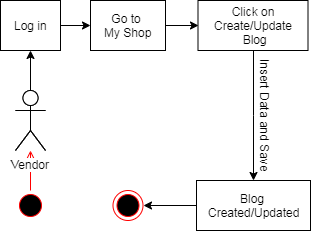
\includegraphics[scale=1]{MyBlog.png}
  \centering
\end{figure}
\begin{figure}
  \caption{UseCase 7: Check Sale History of your products}
  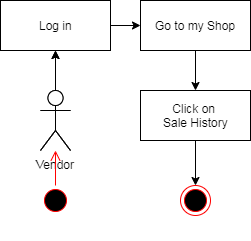
\includegraphics[scale=1]{SalesHistory.png}
  \centering
\end{figure}
\begin{figure}
  \caption{UseCase 8: View reviews and ratings of your Product}
  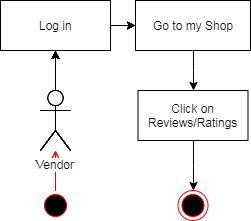
\includegraphics[scale=1]{Ratings.png}
  \centering
\end{figure}
\begin{figure}
  \caption{UseCase 9: Add Skillset to your profile}
  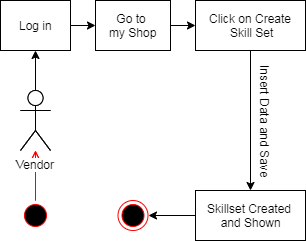
\includegraphics[scale=1]{Skillset.png}
  \centering
\end{figure}
\begin{figure}
  \caption{UseCase 10: Edit/Update your Skillset on the profile}
  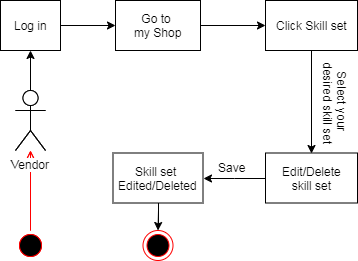
\includegraphics[width=0.75\textwidth]{EditSkillset.png}
  \centering
\end{figure}
\begin{figure}
  \caption{UseCase 11: Customer Registration and subscription to Newsletter}
  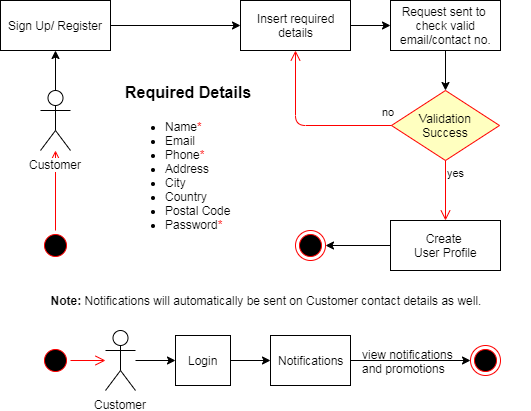
\includegraphics[width=0.75\textwidth]{Register&Notifications.png}
  \centering
\end{figure}
\begin{figure}
  \caption{UseCase 12: Edit/Update an existing Product}
  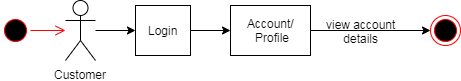
\includegraphics[width=0.75\textwidth]{customer_account_page.png}
  \centering
\end{figure}
\begin{figure}
  \caption{UseCase 13: Edit/Update an existing Product}
  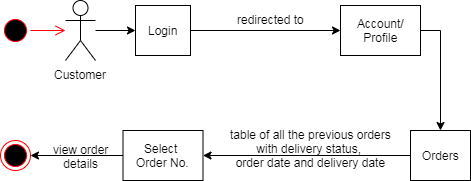
\includegraphics[width=0.75\textwidth]{OrderHistory.png}
  \centering
\end{figure}
\begin{figure}
  \caption{UseCase 14: Edit/Update an existing Product}
  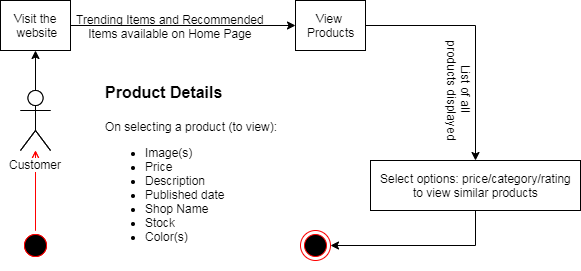
\includegraphics[width=0.75\textwidth]{ViewAllProducts.png}
  \centering
\end{figure}
\begin{figure}
  \caption{UseCase 15: Edit/Update an existing Product}
  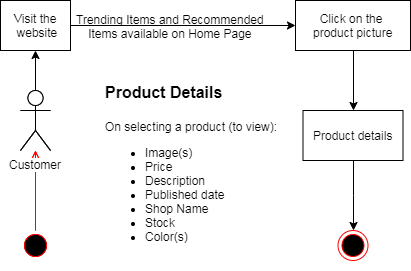
\includegraphics[width=0.75\textwidth]{ViewProduct.png}
  \centering
\end{figure}
\begin{figure}
  \caption{UseCase 16: Edit/Update an existing Product}
  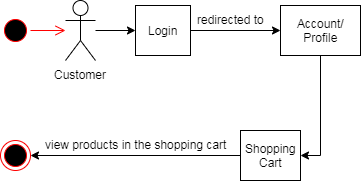
\includegraphics[width=0.75\textwidth]{ShoppingCart.png}
  \centering
\end{figure}


\section{Datasets}
Dummy Data will be generated online and used to populate the Database. There is no particular available dataset for this project.

\section{System Diagram}
This diagram gives a high-level view of the different components of our system and the interactions between them.
The tools and technologies to be used in the system are:
\begin{outline}
    \1 HTML/CSS/Javascript, React and Bootstrap for front-end
    \1 JQuery, Nodejs, and its modules such as Expressjs and Passportjs for back-end
    \1 MongoDB for database
    \1 Amazon Web Services for hosting
    \1 React native for mobile app development
\end{outline}
The module Registration and User Account Portal will be using Passportjs extensively for user authentication, maintaining user sessions and such. The other tools and technologies will be utilized by all modules across the board.
    The system diagram for our system is placed on the next page.

\begin{figure}
  \caption{System Diagram}
  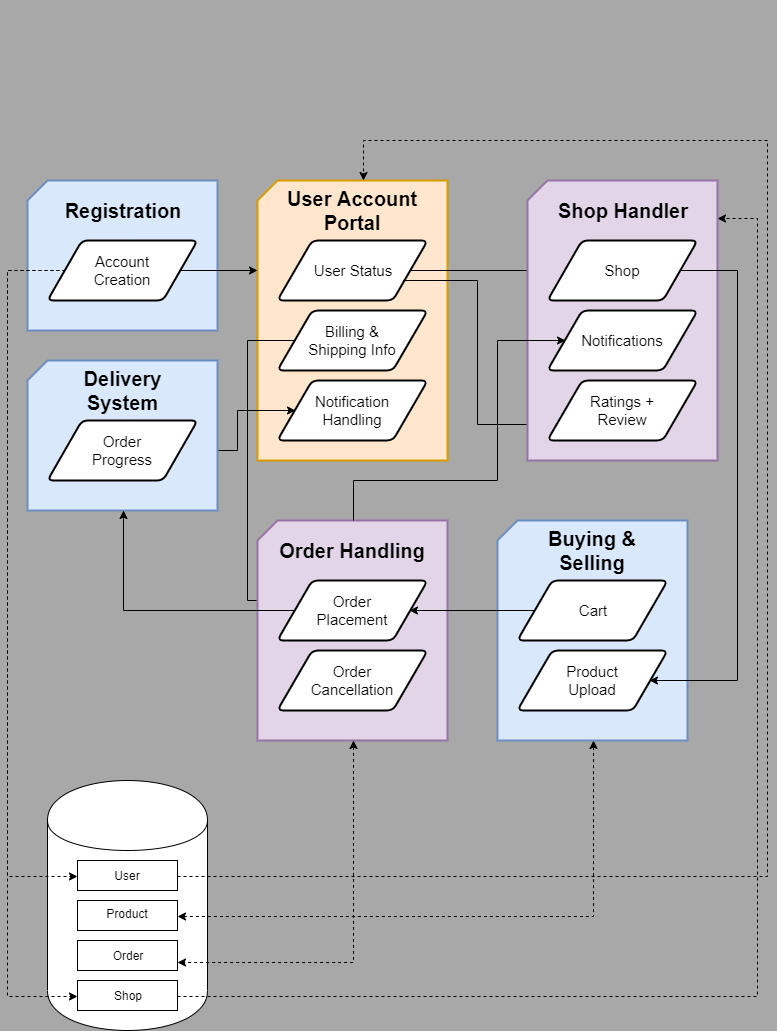
\includegraphics[width=0.75\textwidth]{System_Diagram.png}
  \centering
\end{figure}

\chapter{Software Design Specification (SDS)}
\label{chap:sds}
This chapter provides important artifacts related to design of our project.

\section{Software Design}

This section presents the UML class diagram and gives a brief description of each class in our system. Attributes and methods of each class and relationship among classes are clearly presented.

\begin{figure}
  \caption{UML Class Diagram: The Third Space}
  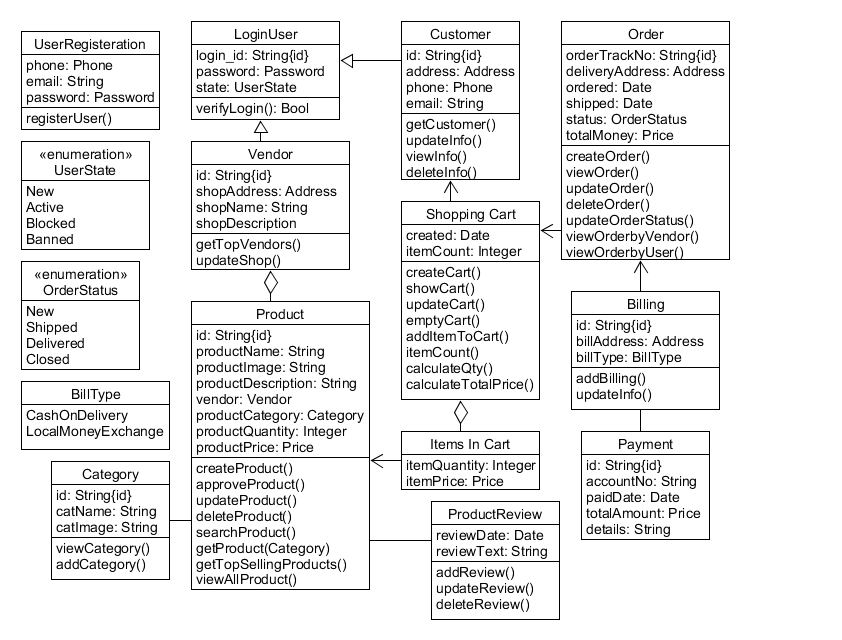
\includegraphics[width=1.25\textwidth]{TheThirdSpaceUML.png}
  \centering
\end{figure}

% Your report will contain ONE of the following 2 sections.

\section{Data Design}

This section presents the structure of our database that caters to persistent data storage in our project. The structure is shown as a normalized data model for relational databases. It clearly shows entities, attributes, relationships with their cardinalities, and primary and foreign keys. We have used DB designer (or any other similar data modeling tool) to build our data model.
\begin{figure}
  \caption{ERD: The Third Space}
  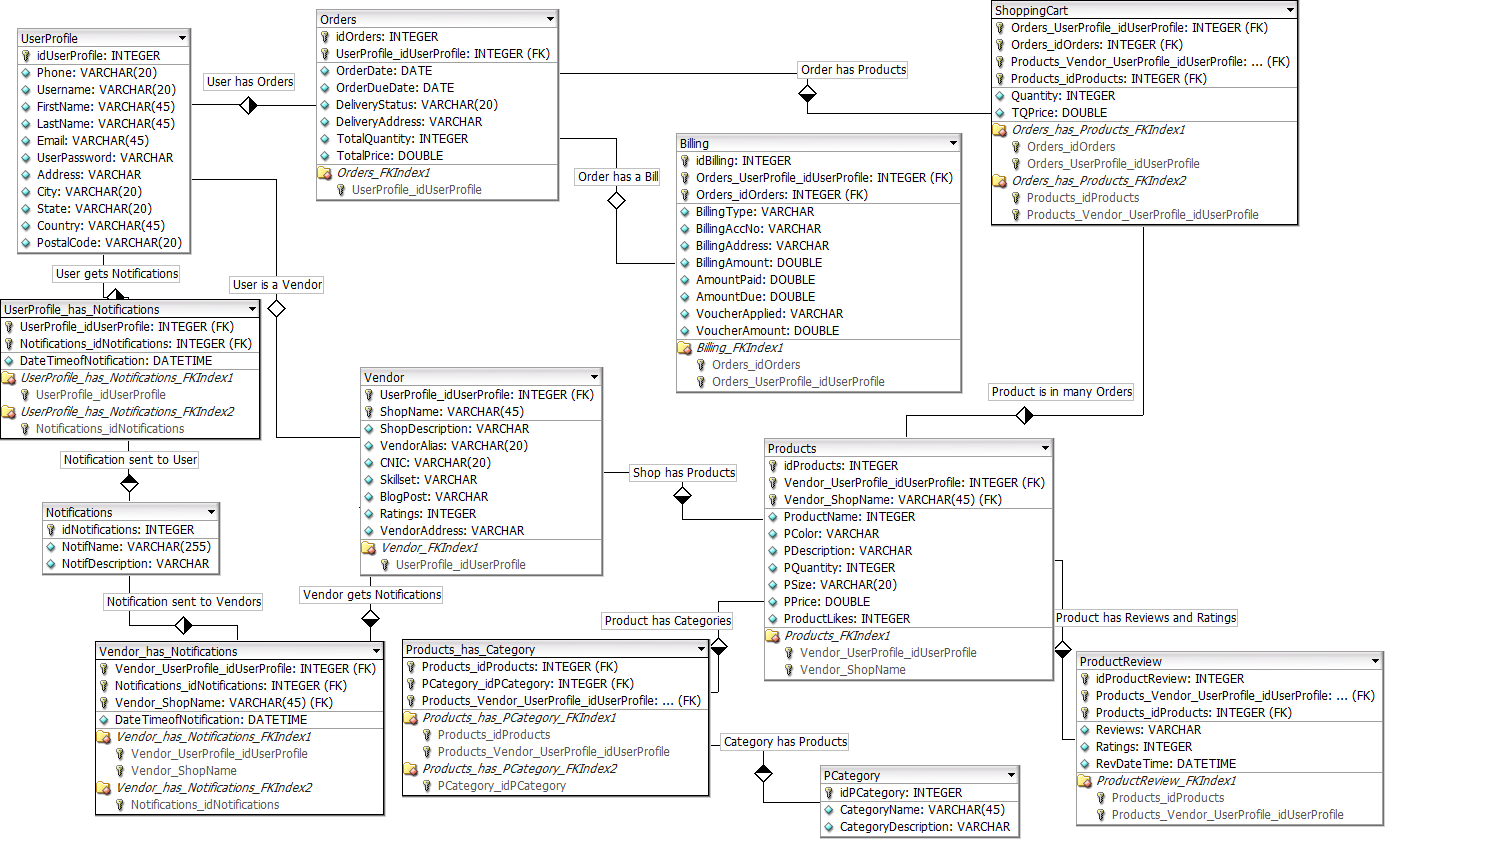
\includegraphics[width=1.25\textwidth]{TheThirdSpaceERD.png}
  \centering
\end{figure}

\chapter{Experiments and Results}
\label{chap:results}
TBA.

\chapter{Conclusion and Future Work}
\label{chap:outro}
TBA.

\begin{appendices}

\titleformat{\chapter}[hang]{\bf\huge}{Appendix \thechapter.}{2pc}{}
% \titleformat{\chapter}[hang]{\bf\huge}{\thechapter.}{2pc}{}

  
% This appendix is optional.
%\chapter{More Math}
%Here, we describe the background math for the techniques used in the text.

% This appendix is required if the data set is not fully described in the main text.
\chapter{User Interface}
Here are some snippets of our project UI
\\\\\textbf{Website:}
    \begin{figure}[h]
        \caption{Website Product UI}
        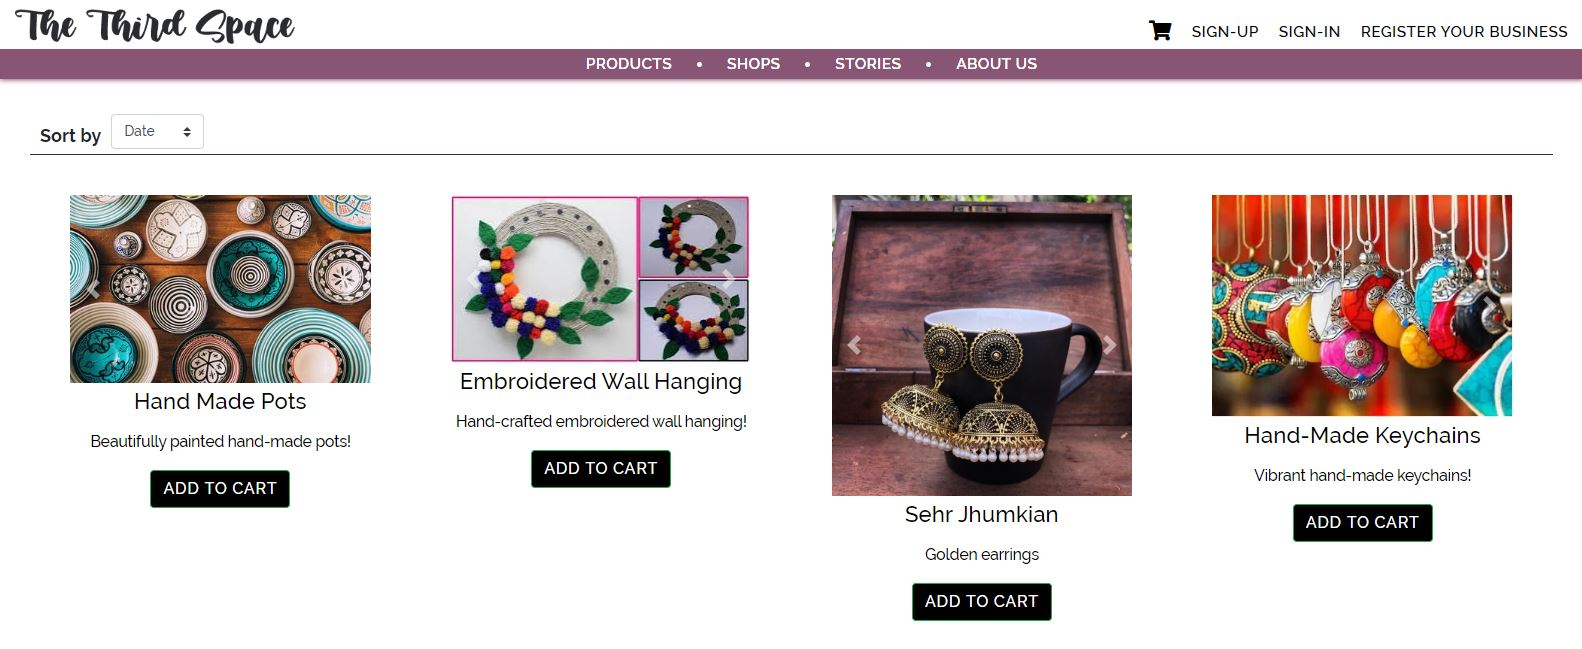
\includegraphics[width=0.75\textwidth]{Web-ProdUI.JPG}
        \centering
    \end{figure}
    \\
    \begin{figure}[h]
        \caption{Website Vendor Registration UI}
        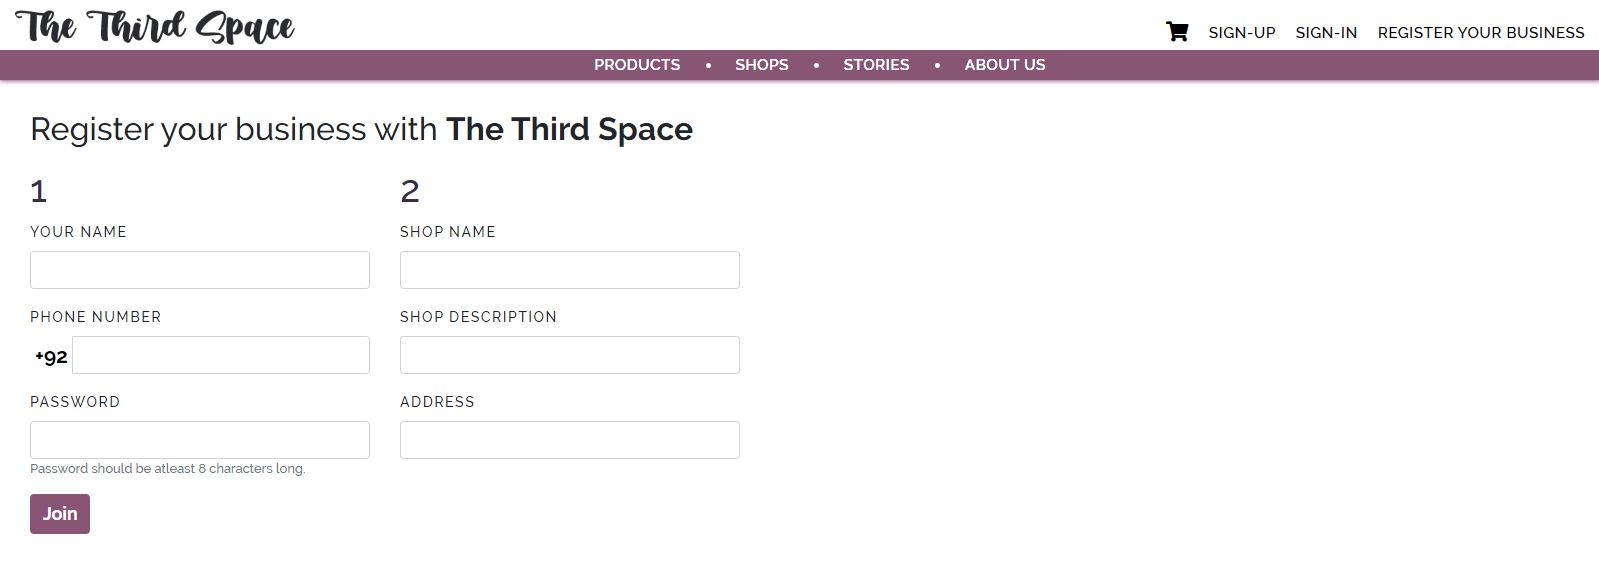
\includegraphics[width=0.75\textwidth]{Web-regUI.JPG}
        \centering
    \end{figure}
\newpage
\textbf{Mobile App:}
    \begin{figure}[ht!]
        \caption{Mobile UI}
        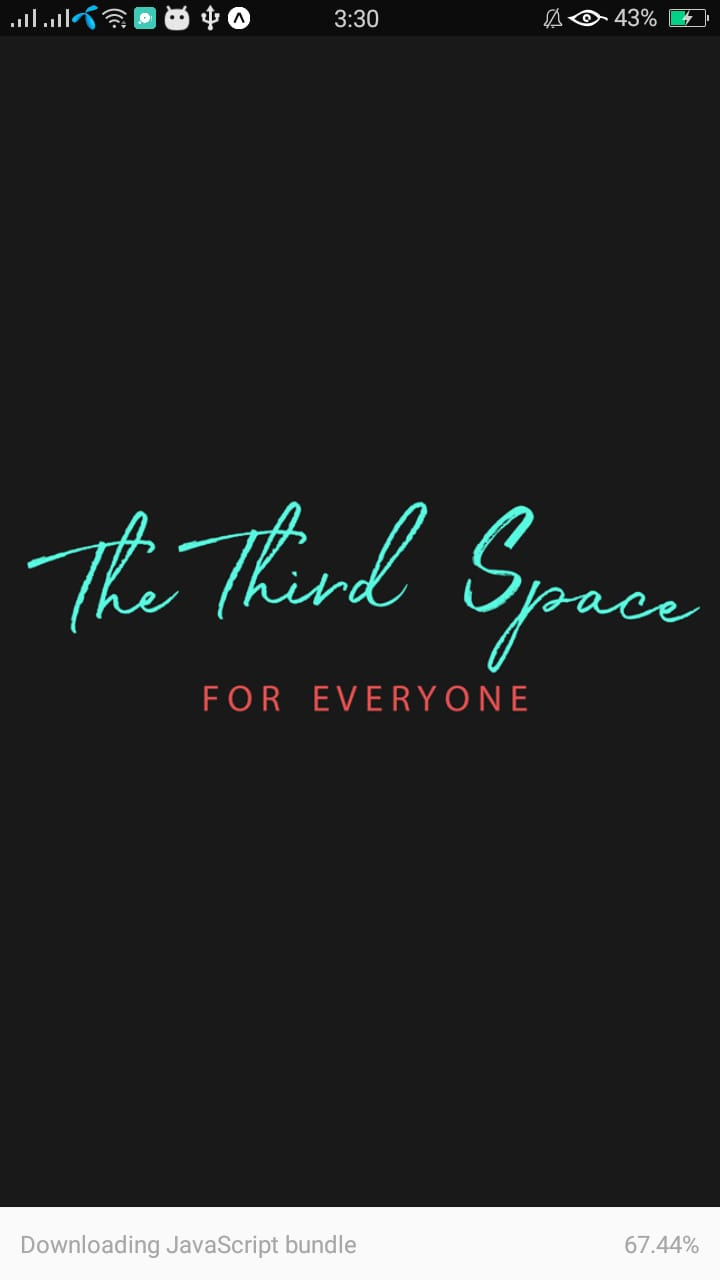
\includegraphics[width=.3\textwidth]{mob3.jpeg}\hfill
        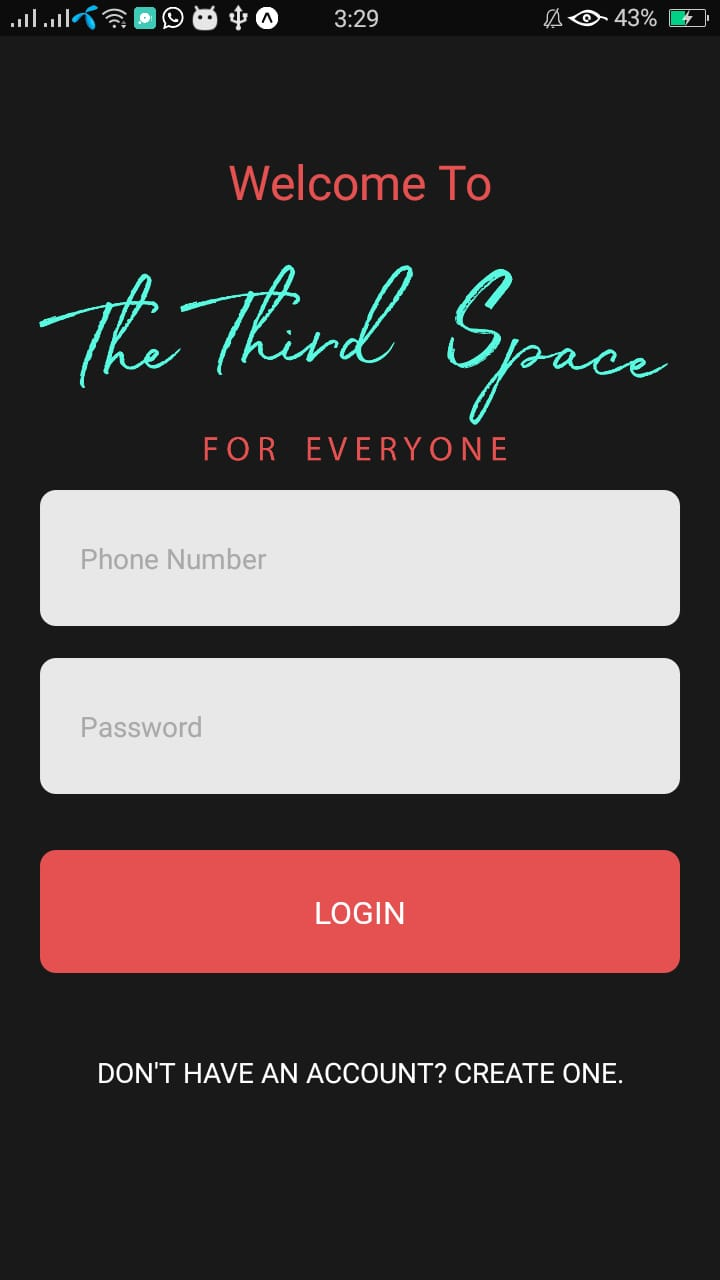
\includegraphics[width=.3\textwidth]{mob2.jpeg}\hfill
        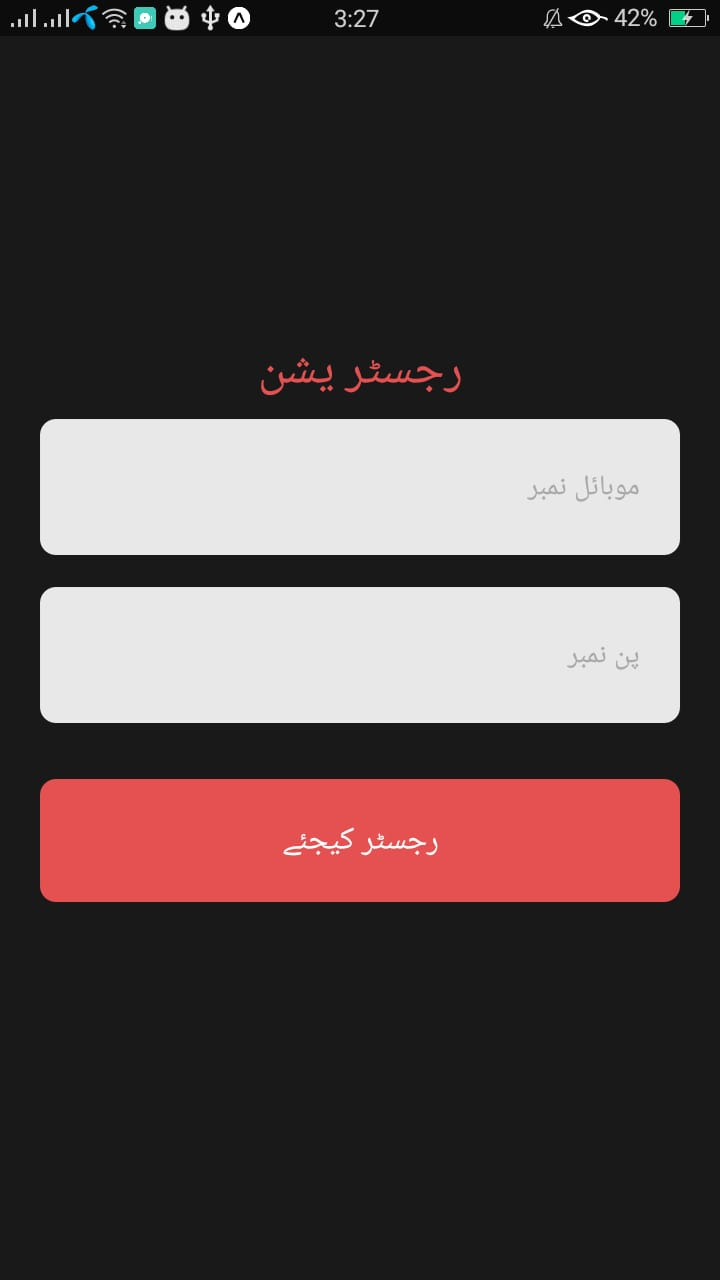
\includegraphics[width=.3\textwidth]{mob1.jpeg}
    \end{figure}

% This appendix is required if the code is not fully described in the main text.
\chapter{Code}
Here is our code. Bits over trees, courtesy of HEC!

% inspired by https://xkcd.com/221/
\begin{lstlisting}[language=python, showstringspaces=false,frame=single]
  print('Hello World!')
  print('Computing true random number.')
  print('Capturing interstellar radiation.')
  print('This will take time!')
  import random
  import time
  time.sleep(3600*random.randint(1,10))
  print(4)
\end{lstlisting}

% Alternately...
Our code can be found at \href{https://github.com/habib-university/Kaavish-Template}{this GitHub link}.

%%% Local Variables:
%%% mode: latex
%%% TeX-master: "../report"
%%% End:

\end{appendices}

% Print the bibliography with a ToC entry and titled, "References".
\printbibliography[heading=bibintoc,title={References}]

\end{document}

%%% Local Variables:
%%% mode: latex
%%% TeX-master: t
%%% End:
